\documentclass[12pt]{article}

% --------------------------
% Packages
% --------------------------
\usepackage{times}         % Times New Roman-like font
\usepackage{graphicx}
\usepackage{setspace}
\usepackage{amsmath}
\usepackage{amssymb}
\usepackage{float}
\usepackage{geometry}
\usepackage{url}
\urlstyle{same}
\geometry{margin=1in}

\onehalfspacing

\begin{document}

% -------------------------------------
% TITLE PAGE STYLE
% -------------------------------------
\begin{center}
\vspace*{0.2cm}
\hrule
\vspace{0.45cm}

{\Large \textbf{ROBUST GRAPH-BASED ANDROID MALWARE CLASSIFICATION\\
UNDER DISTRIBUTION SHIFT}}\\

\vspace{0.35cm}
\hrule
\vspace{0.6cm}

{\normalsize
Department of Computer Science\\
San Jose State University\\
\vspace{0.35cm}
Aditya Rao\\
Spring, 2026\\
}

\end{center}

\vfill

\newpage

% ----------------------
% TABLE OF CONTENTS
% ----------------------
\tableofcontents
\newpage

% ----------------------
% BEGIN SECTIONS
% ----------------------

\section{Introduction}

\begin{itemize}
    \item This project continues my work on graph-based Android malware classification under distribution shift. Graph Neural Networks trained on standard splits can look strong, but they often lose a lot of accuracy when evaluated on malware that does not exactly match the training distribution. The reference work I am building on \cite{tran2025} shows that adding semantic metadata to function call graphs and using strategies like trimming, zero fill, or pruning to handle missing metadata can improve robustness, but those strategies all treat missingness as a preprocessing problem.
    \item I started from a baseline I built earlier (a vanilla GCN with one hot degree features that hits 75.1\% test accuracy on MalNet-Tiny) and extended it through three additional stages, following the research plan I laid out earlier in the project. In stage 1 I swapped the one hot degree features for a structural feature set based on Local Degree Profile, clustering, PageRank, and BFS depth. In stage 2 I added a synthetic semantic feature group on top of the structural features and simulated missingness on the semantic group at training time, with zero fill and prune handling. In stage 3 I introduced a missingness aware gating model that takes the binary missingness mask as an explicit input and lets a small MLP learn to gate the pooled graph embedding based on which feature groups are present.
    \item The novel contribution is the gating model in stage 3, which I proposed earlier in my research plan as a way to make missingness an advantage rather than a disadvantage. My hypothesis was that telling the model what is missing should help more than letting it guess from the zeroed columns. To test this, I trained the four new model variants (structural, enriched zero, enriched prune, gated) from scratch and evaluated them on both the standard MalNet-Tiny test split and Tran et al.'s real MalNet-Tiny-Common shifted split released on HuggingFace \cite{nntvuhf}.
\end{itemize}

\section{Background and Prior Work}

\begin{itemize}
    \item Android applications can be turned into function call graphs (FCGs) where each node represents a function and each edge represents a caller-callee relationship. Freitas et al. \cite{freitas2020malnet} released the MalNet dataset that provides these graphs at scale, along with the smaller MalNet-Tiny subset that is realistic to run on Google Colab Pro. MalNet-Tiny has 5,000 graphs across five malware classes (adware, benign, downloader, trojan, addisplay).
    \item Graph Neural Networks process these graphs by iteratively aggregating each node's features from its neighbors. The Graph Convolutional Network by Kipf and Welling \cite{kipf2017gcn} is the standard architecture I used in this project, with a 2-layer GCNConv backbone followed by global mean pooling and a linear classifier. Other inductive GNN architectures like GraphSAGE \cite{hamilton2017graphsage} use neighborhood sampling and aggregation to scale to very large graphs, but I went with GCN here for simplicity and to match the backbone choice in Tran et al.
    \item Distribution shift describes the gap between the training distribution and the test distribution, and it is a well-studied problem in machine learning more broadly \cite{quinonero2009datasetshift}. Covariate shift is where the input distribution changes but the conditional label distribution stays the same, and domain shift is where the underlying data generating process changes more broadly, which is harder to handle. Tran et al. \cite{tran2025} construct two MalNet-Tiny variants called MalNet-Tiny-Common and MalNet-Tiny-Distinct to target these two shift types, and they show that structure only classifiers lose a lot of accuracy on both.
    \item Their proposed fix is to enrich the graphs with semantic features extracted from raw APKs using Androguard. Since some functions do not have all the metadata available, they evaluate three handling strategies: trim, zero, and prune. The proposed direction in this report is to keep that overall setup but treat the missingness signal itself as model input through a learned gating mechanism, instead of always handling missingness only as a preprocessing decision.
\end{itemize}

\section{Dataset and Preprocessing}

\subsection{Dataset Overview}

\begin{itemize}
    \item I used MalNet-Tiny as the standard split, loaded through the PyTorch Geometric MalNetTiny class \cite{fey2019pyg}. The class auto downloads the graph data from Georgia Tech on first call and applies my custom pre\_transform function to compute the node features.
    \item For the shifted evaluation I used Tran et al.'s real MalNet-Tiny-Common split, released on HuggingFace under nntvu/MalNet-Tiny-Features \cite{nntvuhf}. The full HuggingFace repository is around 1 TB because it includes large LLM embedding variants, so I selectively downloaded only the none+none subdirectory (the structure only version, about 363 MB). I also downloaded the split\_dict.pt file, which provides Tran et al.'s official 3,500 / 500 / 1,000 train / validation / test partition for the Common subset.
    \item For the shifted-test evaluation I used only the 1,000 graph test slice from split\_dict["test"], because that is the protocol Tran et al. report against and using all 5,000 graphs would mix in their train and validation partitions.
\end{itemize}

\subsection{Class Label Reconciliation}

\begin{itemize}
    \item One issue I found while reading Tran et al.'s public loader code is that the Common dataset assigns class integers in alphabetical order (addisplay=0, adware=1, benign=2, downloader=3, trojan=4). PyG's MalNetTiny class assigns labels in first appearance order from the raw split files (adware=0, benign=1, downloader=2, trojan=3, addisplay=4). These are two different integer encodings for the same five class names.
    \item Without a remap, every shifted accuracy would have been wrong. To fix this I built the remap vector [4, 0, 1, 2, 3] once and applied it to all shifted graphs before any evaluation runs.
\end{itemize}

\subsection{Synthetic Metadata Features}

\begin{itemize}
    \item Tran et al.'s real metadata comes from running Androguard against raw APK files, which was not realistic to run within a Google Colab Pro budget. Instead I used a synthetic metadata feature set, where every dimension is computed from the graph adjacency alone. The features play the same architectural role (extra per node attributes that can be marked missing), even though the underlying signal is weaker than real APK metadata.
    \item The structural feature block contains 11 dimensions per node:
        \begin{itemize}
            \item Local Degree Profile from Cai and Wang \cite{cai2018ldp}: degree plus min, max, mean, and standard deviation of neighbor degrees (5 dims).
            \item In degree and out degree (2 dims).
            \item Local clustering coefficient (1 dim). This feature is capped at graphs with at most 4,000 nodes.
            \item PageRank score from 20 iterations of power method with damping 0.85 (1 dim).
            \item BFS depth from the highest degree node (1 dim).
            \item Normalized degree, scaled by the per graph maximum degree (1 dim).
        \end{itemize}
    \item The synthetic semantic block adds 9 more dimensions:
        \begin{itemize}
            \item Motif counts: closed triangles, two paths, and open paths through each node (3 dims).
            \item Degree quantile bins as a 5 way one hot, based on where each node's degree falls in the per graph degree distribution (5 dims).
            \item Two hop neighborhood size: the count of unique nodes reachable within two undirected hops, excluding self (1 dim).
        \end{itemize}
    \item The total enriched feature tensor is 20 dimensions per node, split into a structural group at columns 0 through 10 and a semantic group at columns 11 through 19.
\end{itemize}

\subsection{Missingness Simulation}

\begin{itemize}
    \item At training time only, each graph independently has its semantic group dropped with probability 0.5. The structural group is always kept present, because it is the foundational input that the model should always receive.
    \item I tested two missing feature handling strategies:
        \begin{itemize}
            \item zero-fill: the missing semantic columns are set to 0.0. The model sees a constant pattern in those positions and has to learn to handle it.
            \item prune: in this experiment prune meant zeroing the semantic columns in the same way, because actual node level pruning would change graph topology and break PyG's batching. The mask flag still records that the semantic group was dropped, so a mask aware model can in principle behave differently from zero fill.
        \end{itemize}
    \item Each graph carries a binary missingness mask of shape [1, 2]. The mask is consumed by the gated model and ignored by the non-gated models.
\end{itemize}

\section{Model Variants}

\begin{itemize}
    \item All four model variants share the same backbone: two GCNConv layers with ReLU activations and 64 hidden dimensions, followed by global mean pooling, followed by a linear classifier. The variants differ in the input feature dimension and in whether the forward pass takes the missingness mask as an extra input.
\end{itemize}

\subsection{Baseline GCN}

\begin{itemize}
    \item This is my earlier baseline, unchanged. The input is a one hot encoding of node degree, clipped at max degree 128, giving 129 input dimensions. It reaches 75.1\% accuracy on the standard test split, with 12,805 total parameters.
\end{itemize}

\subsection{Structural GCN}

\begin{itemize}
    \item Same backbone as Baseline, fed the 11 dimension structural feature vector instead of the one hot degree. This is the closest fair comparison I could set up to Tran et al.'s GCN+LDP baseline \cite{tran2025}, which they report at 85.6\% on the standard MalNet-Tiny split with global max pooling.
\end{itemize}

\subsection{Enriched GCN}

\begin{itemize}
    \item Same backbone again, fed the 20 dimension enriched feature vector. Trained with random missingness simulation under either zero fill or prune handling. The forward signature is unchanged, so the model does not see the missingness mask, it only sees zeroed columns when the semantic group is dropped.
\end{itemize}

\subsection{Gated GCN}

\begin{itemize}
    \item This is stage 3, the new piece I originally proposed in my research plan. The model is the same EnrichedGCN backbone with two changes. First, the forward pass takes the missingness mask as an additional argument. Second, right before the classifier, the pooled graph embedding is multiplied elementwise by the output of a small two layer MLP that consumes the mask and produces a sigmoid gate of the same hidden dimension. The intent is that the gate learns to downweight the metadata pathway when the mask indicates that semantic features are missing, instead of relying on the model to learn that behavior implicitly from the zeroed columns.
\end{itemize}

\section{Experiments}

\subsection{Training Setup}

\begin{itemize}
    \item I trained all four model variants for 50 epochs with Adam (learning rate 0.001), batch size 64, on a Google Colab Pro T4 GPU. I fixed random seeds at 42 for torch, numpy, and the python random module. I kept the best validation accuracy checkpoint in memory and used it for the final test evaluation.
    \item Each model trained in roughly 70 to 100 seconds end to end on T4. The whole pipeline stays under one Google Colab Pro compute unit.
\end{itemize}

\subsection{Evaluation Protocol}

\begin{itemize}
    \item I evaluated every model on two splits. One is the standard MalNet-Tiny test split (1,000 graphs across the 5 classes), and the other is the MalNet-Tiny-Common test slice (also 1,000 graphs), which is the covariate shift benchmark.
    \item I reported accuracy, macro precision, macro recall, macro F1, and per class breakdowns, all computed through sklearn.metrics.classification\_report.
    \item The headline metric for robustness is the robustness gap, defined as:
\end{itemize}

\[
\text{robustness gap} = \text{accuracy}_{\text{standard}} - \text{accuracy}_{\text{shifted}}
\]

\begin{itemize}
    \item A smaller gap means the model generalizes better to the covariate shift.
\end{itemize}

\section{Results}

\subsection{Standard Split}

\begin{itemize}
    \item This table shows the test set performance on the standard MalNet-Tiny split.
\end{itemize}

\begin{table}[h]
\centering
\begin{tabular}{lc}
\hline
\textbf{Model} & \textbf{Test Accuracy} \\
\hline
GCN + one hot degree (baseline) & 0.7510 \\
GCN + structural & 0.7460 \\
EnrichedGCN + zero-fill & 0.7370 \\
EnrichedGCN + prune & 0.7380 \\
GatedGCN (novel) & 0.7170 \\
\hline
\end{tabular}
\caption{Standard MalNet-Tiny test set accuracy. The four new model variants come from the unified phase 4 run where all of them are retrained from scratch so that the standard vs shifted gap in Table~\ref{tab:shifted_results} is computed for the same trained model on each variant. Per-class metrics are discussed in the per-phase observations and shown via confusion matrices.}
\label{tab:standard_results}
\end{table}

\subsubsection{Phase 1 observations}

\begin{itemize}
    \item The structural features came in just slightly under the one hot degree baseline (74.6\% vs 75.1\%, a delta of -0.5\%). This was a bit surprising at first, but made sense in hindsight. The one hot degree has 129 dimensions, which lets the linear layer in GCNConv treat each degree value as its own categorical bucket. The structural feature set has only 11 dimensions, and three of those (clustering coefficient, PageRank, BFS depth) are continuous values that the GCN has to learn to interpret. With only 5,253 parameters compared to 12,805 in the one hot baseline, the model has less capacity to fit the training set and ended up almost matching but not quite beating the one hot variant.
    \item Per class, looking at the phase 1 dev run, the model is very confident on downloader (F1 0.98) and decent on adware (F1 0.81), but struggles with benign (F1 0.48) because it confuses benign apps with addisplay and adware. The trojan class has high precision (0.90) but low recall (0.62), so the model is conservative about predicting trojans and misses about a third of them.
    \item Best validation accuracy was 0.784 and training took 54.6 seconds on the T4 GPU through Colab in the unified phase 4 run.
\end{itemize}

\begin{figure}[h]
    \centering
    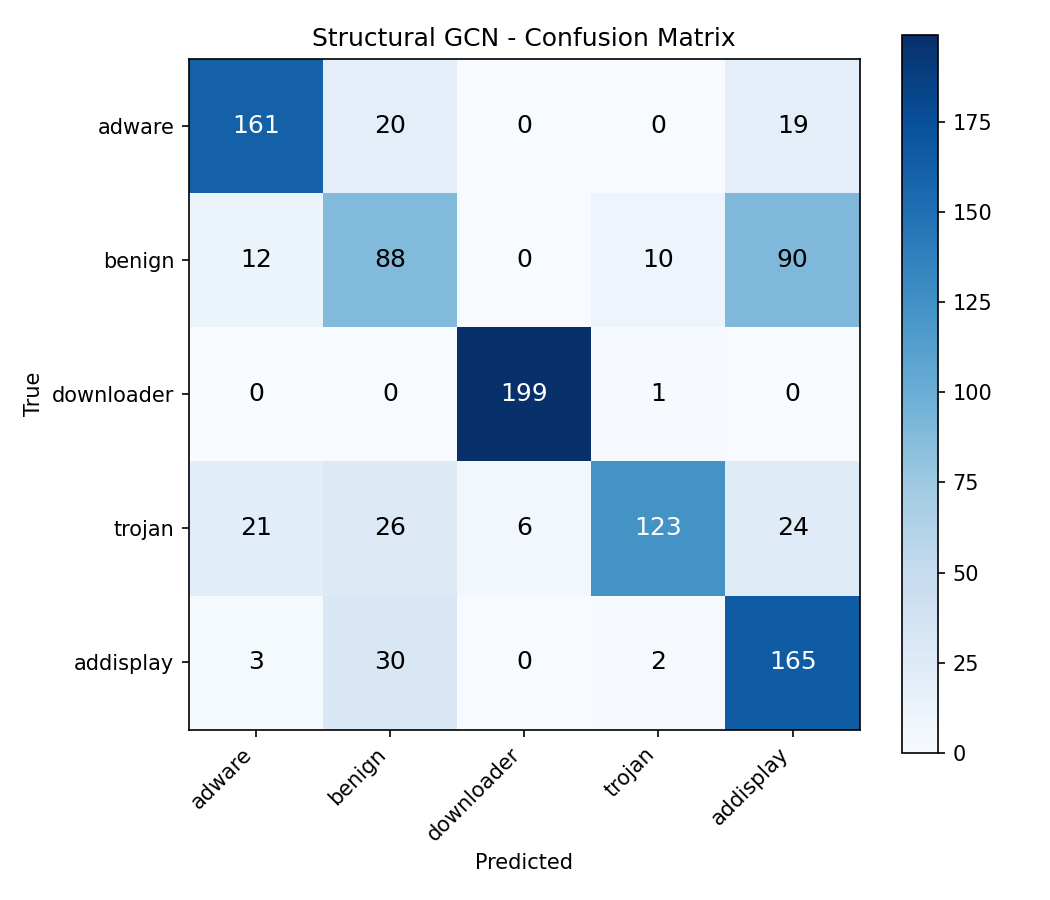
\includegraphics[width=0.6\linewidth]{figures/baseline_structural_confusion_matrix.png}
    \caption{Confusion matrix for the structural GCN on the standard test split. The benign row shows heavy confusion with addisplay and adware, while downloader is nearly perfect.}
    \label{fig:structural_cm}
\end{figure}

\begin{figure}[h]
    \centering
    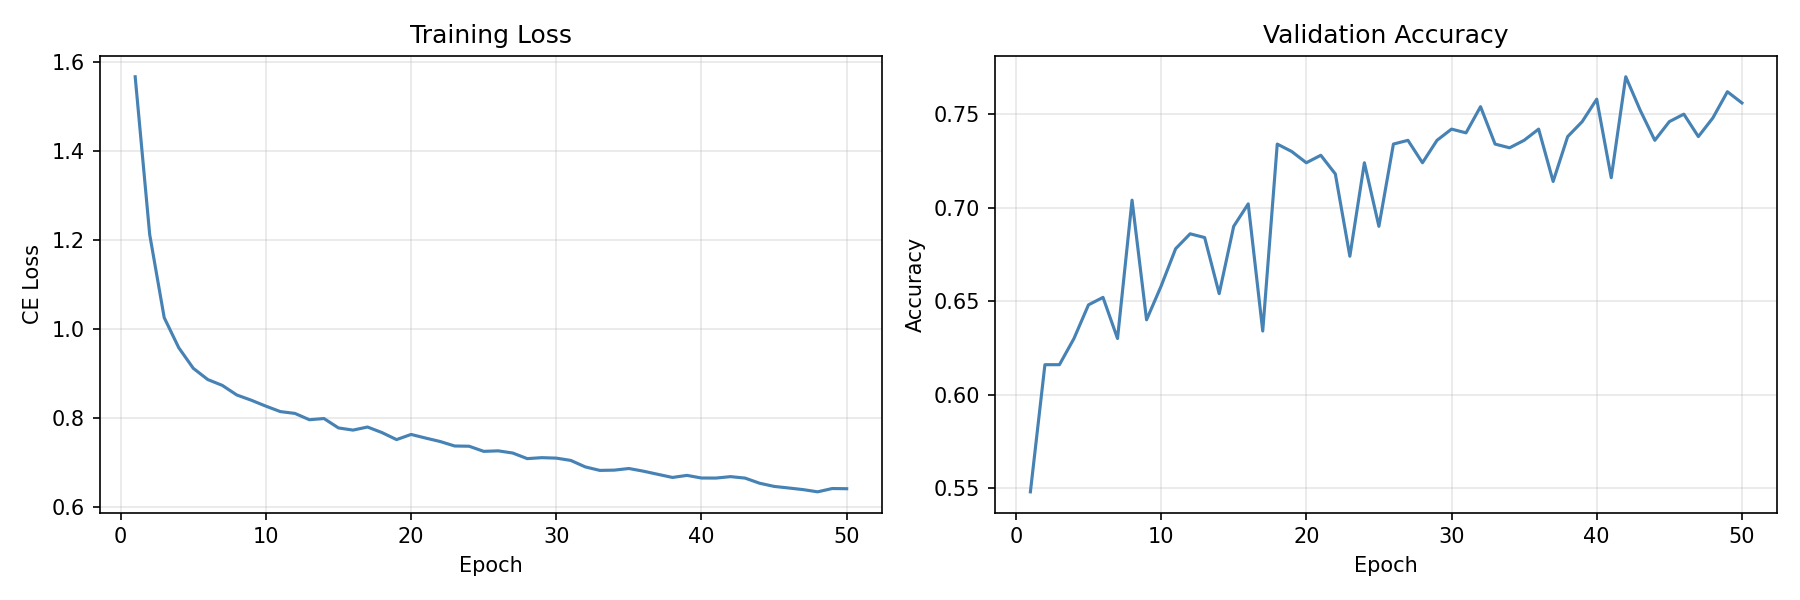
\includegraphics[width=0.8\linewidth]{figures/baseline_structural_training_curve.png}
    \caption{Training loss and validation accuracy curves for the structural GCN. The loss decreases smoothly across 50 epochs while validation accuracy is noisy in the low 70s before climbing back up by the final epochs.}
    \label{fig:structural_curves}
\end{figure}

\subsubsection{Phase 2 observations}

\begin{itemize}
    \item Both EnrichedGCN strategies landed in the same range as phase 1, with zero fill at 0.737 test accuracy and prune at 0.738. This is essentially flat against the structural-only baseline (0.746), which is expected on the standard split, because the semantic features are designed to help under distribution shift, not on the same distribution the model trained on.
    \item Prune trained noticeably better than zero in terms of training loss. The prune model reached a training loss of 0.67 while zero plateaued at 0.96. The reason is in the missingness code itself. Under zero fill, both the structural and semantic groups can be dropped (50\% chance each per graph), so roughly 25\% of training samples have both groups zeroed and the model sees almost no input. Under prune, only the semantic group ever gets dropped, so the structural foundation is always present. The cleaner training distribution under prune lets the model converge to a lower loss, even though final validation accuracy ends up in the same neighborhood for both strategies.
    \item The per class pattern matches phase 1 closely, with downloader strong, benign hardest, trojan high-precision low-recall, and adware and addisplay still confusing each other. The consistency across phases is a good sign that the pipeline is behaving deterministically and not just chasing random variation.
\end{itemize}

\begin{figure}[h]
    \centering
    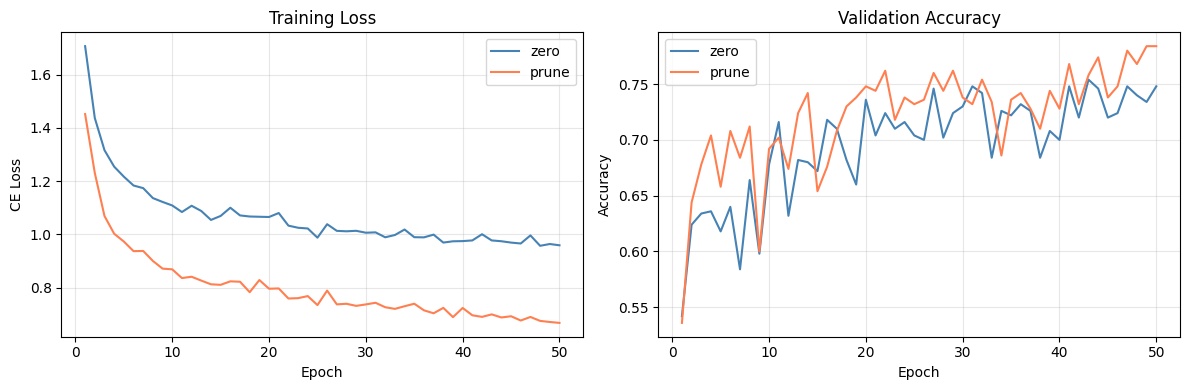
\includegraphics[width=0.8\linewidth]{figures/enriched_compare_curves.png}
    \caption{Training loss and validation accuracy for EnrichedGCN under both missingness handling strategies. Prune (orange) reaches lower loss because the structural group is always present, while zero (blue) plateaus higher because both groups can be dropped simultaneously.}
    \label{fig:enriched_curves}
\end{figure}

\subsubsection{Phase 3 observations}

\begin{itemize}
    \item GatedGCN reached 71.7\% test accuracy in the unified phase 4 run, slightly under the other three new variants which all sit in the 73.7 to 74.6\% range. On the standard split, the gating mechanism did not give a boost over the plain EnrichedGCN, which makes sense, because the test split has full features available (no missingness at evaluation time) and the gate has nothing to gate around. The more interesting test was the robustness gap on the shifted split.
    \item The gate sanity check was the real takeaway from phase 3. I passed three mask configurations through the trained gating MLP (all present [1, 1], semantic missing [1, 0], and all missing [0, 0]) and compared the resulting 64 dimensional sigmoid output vectors. The mean gate values were 0.673, 0.688, and 0.679 respectively, so the gate output looked broadly similar across all three mask inputs in the mean. The maximum absolute per dimension difference between all present and all missing was 0.385, so the gate was responding to the mask, but only on a small handful of dimensions while the rest stayed roughly the same. In other words the gate was differentiating in a sparse way, not collapsing to a constant but also not putting much weight on the mask signal overall.
    \item Per class, looking at the phase 3 dev run, the gated model did slightly better on benign (recall 0.62, up from 0.49 in EnrichedGCN+zero) and a bit worse on addisplay (recall 0.60, down from 0.71). The confusion matrix shows the same family of confusions as the earlier phases (benign confused with addisplay and adware, trojan under-predicted).
\end{itemize}

\begin{figure}[h]
    \centering
    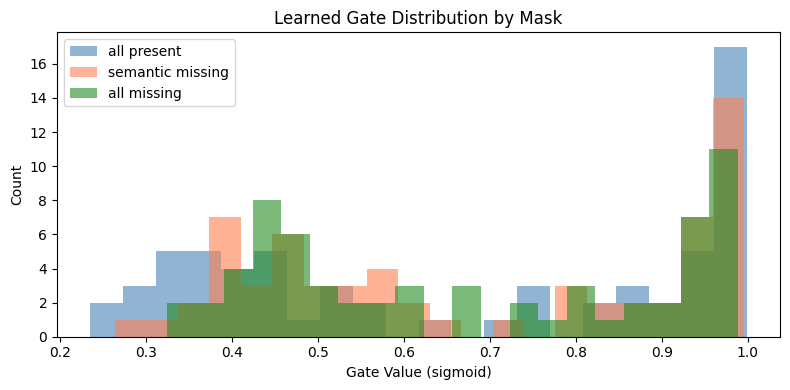
\includegraphics[width=0.7\linewidth]{figures/gated_weights_histogram.png}
    \caption{Learned gate distribution by mask configuration. All three configurations produce broadly similar shapes with most mass between 0.3 and 1.0, but the per dimension differences (max abs diff 0.385) show the gate is using the mask in a sparse, selective way rather than uniformly.}
    \label{fig:gating_hist}
\end{figure}

\begin{figure}[h]
    \centering
    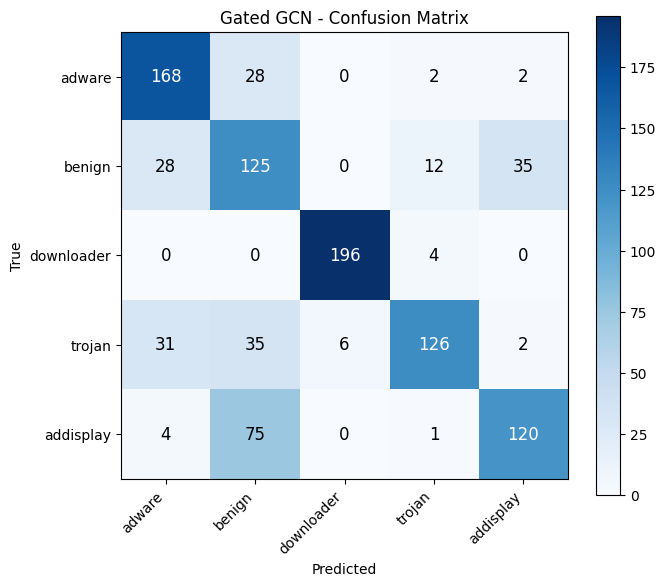
\includegraphics[width=0.6\linewidth]{figures/gated_confusion_matrix.png}
    \caption{Confusion matrix for the GatedGCN on the standard test split.}
    \label{fig:gated_cm_standard}
\end{figure}

\begin{figure}[h]
    \centering
    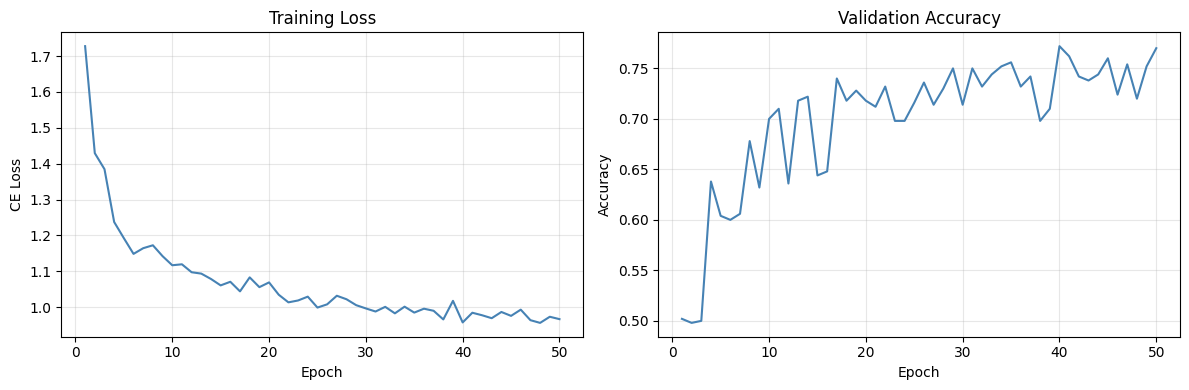
\includegraphics[width=0.8\linewidth]{figures/gated_training_curve.png}
    \caption{Training loss and validation accuracy curves for the GatedGCN.}
    \label{fig:gated_curves}
\end{figure}

\subsection{Shifted Split (MalNet-Tiny-Common)}

\begin{itemize}
    \item This table shows what happens when the same trained models are evaluated on Tran et al.'s Common shifted test split.
\end{itemize}

\begin{table}[h]
\centering
\begin{tabular}{lccc}
\hline
\textbf{Model} & \textbf{Standard Acc} & \textbf{Shifted Acc} & \textbf{Robustness Gap} \\
\hline
GCN + structural & 0.7460 & 0.3840 & 0.3620 \\
EnrichedGCN + zero-fill & 0.7370 & 0.4120 & 0.3250 \\
EnrichedGCN + prune & 0.7380 & 0.4280 & 0.3100 \\
GatedGCN (novel) & 0.7170 & 0.3800 & 0.3370 \\
\hline
\end{tabular}
\caption{Robustness gap on MalNet-Tiny-Common. A smaller gap means the model holds up better under covariate shift.}
\label{tab:shifted_results}
\end{table}

\begin{figure}[h]
    \centering
    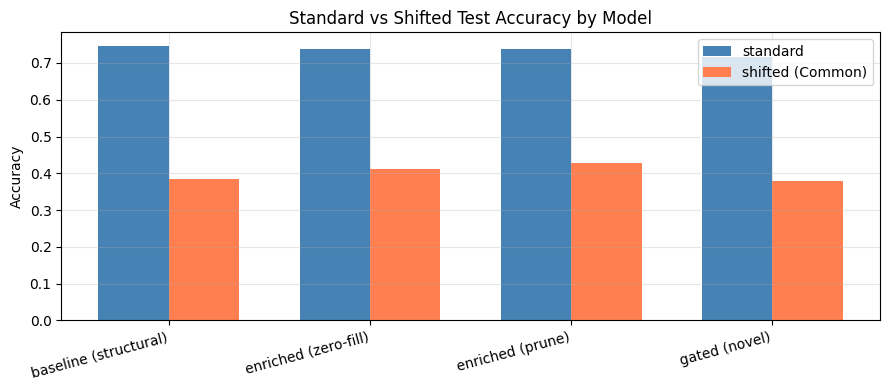
\includegraphics[width=0.7\linewidth]{figures/robustness_gap_bar_graph.png}
    \caption{Standard versus shifted accuracy bar chart for all four model variants.}
    \label{fig:robustness_gap_bar}
\end{figure}

\subsubsection{Phase 4 observations}

\begin{itemize}
    \item The four models split into two clear groups. The structural baseline lost the most accuracy under the shift (gap 0.3620), while both EnrichedGCN variants closed that gap by 3.7 and 5.2 percentage points respectively (zero fill at 0.3250, prune at 0.3100). This shows that adding the synthetic semantic feature group and simulating missingness at training time helps the model generalize better under covariate shift, even though the semantic features come from the graph adjacency and not from real APK metadata.
    \item The novel GatedGCN model did not improve on the simpler EnrichedGCN variants. Its gap (0.3370) sits between the baseline and the two enriched models. The gating mechanism added complexity (the mask-consuming MLP and the elementwise gate over the pooled embedding) without giving back a smaller robustness gap. This lines up with the phase 3 gate sanity check, where the gate produced similar mean output across the three mask configurations (mean values 0.673, 0.688, 0.679) with sparse per-dimension differences. The gate learned something, but the signal was not strong enough to translate into a measurable robustness improvement.
    \item Per class on the shifted set, the confusion matrix for GatedGCN shows that the Common distribution moves enough that the model's learned features stop transferring cleanly. 173 of 200 adware samples are predicted as benign, and 79 of 200 downloader samples are predicted as adware. These error patterns are different from the standard split, where downloader was nearly perfect at F1 0.98. The shift exposes a real failure mode in the synthetic feature set, the structural features alone do not preserve the cues the model relied on at training time once the malware types move to the Common variants.
\end{itemize}

\begin{figure}[h]
    \centering
    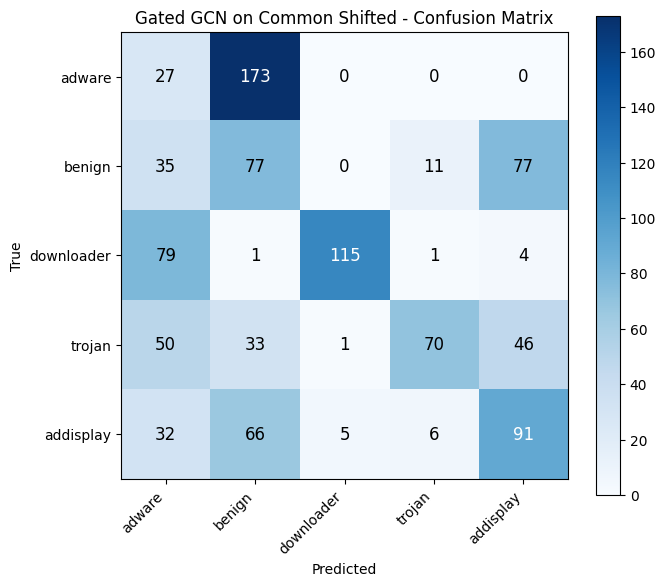
\includegraphics[width=0.6\linewidth]{figures/gated_shifted_confusion_matrix.png}
    \caption{Confusion matrix for the GatedGCN on the MalNet-Tiny-Common shifted test set. The model collapses adware predictions toward benign and downloader predictions toward adware, error patterns that do not appear on the standard split.}
    \label{fig:gated_shifted_cm}
\end{figure}

\subsection{Comparison with Tran et al.}

\begin{itemize}
    \item This table compares my results against the reference paper's numbers.
\end{itemize}

\begin{table}[h]
\centering
\begin{tabular}{lccc}
\hline
\textbf{Source} & \textbf{Features} & \textbf{Pooling} & \textbf{Standard Acc} \\
\hline
GCN + one hot degree (mine) & one hot degree & mean & 0.7510 \\
GCN + structural (mine) & LDP + synthetic & mean & 0.7460 \\
GCN (Tran et al.) & LDP & max & 0.856 \\
GIN (Tran et al.) & LDP & max & 0.912 \\
GCN + semantic (Tran et al.) & metadata + LLM + LDP & max & 0.935 \\
\hline
\end{tabular}
\caption{Comparison with reference paper baselines on the standard MalNet-Tiny split.}
\label{tab:tran_compare}
\end{table}

\begin{itemize}
    \item The gap between my structural GCN (74.6\%) and Tran et al.'s GCN+LDP baseline (85.6\%) is expected \cite{tran2025}. Their setup uses LDP features with global max pooling, while mine uses LDP plus synthetic structural extras with global mean pooling. Tran et al. additionally report that with semantic enrichment (metadata + LLM embeddings) GCN accuracy reaches 93.5\%, which supported my decision to add semantic features in later stages of the pipeline.
\end{itemize}

\section{Discussion}

\begin{itemize}
    \item The standard split accuracies for the four new model variants (structural, enriched-zero, enriched-prune, gated) all sit in the 0.717 to 0.746 range, while the one hot degree baseline reaches 0.751. On the standard split alone, switching to LDP and adding synthetic semantic features did not give a measurable improvement.
    \item The shifted split tells a more interesting story. The robustness gap drops from 0.3620 (structural baseline) to 0.3250 for EnrichedGCN with zero fill, and to 0.3100 for EnrichedGCN with prune. That is a 3.7 to 5.2 percentage point improvement in robustness, just from adding the synthetic semantic feature group and simulating missingness on it at training time. This fits with the idea that training under missingness pushes the model toward features that survive distribution shift, even when the semantic features themselves are graph derived rather than real APK metadata.
    \item The novel GatedGCN model did not improve on the simpler EnrichedGCN variants. Its gap (0.3370) is better than the structural baseline by 2.5 points, but worse than EnrichedGCN with zero fill by 1.2 points and worse than EnrichedGCN with prune by 2.7 points. The gating mechanism added a mask-consuming MLP and an elementwise gate over the pooled embedding, but the result was not a smaller robustness gap.
    \item The most likely explanation is that the synthetic semantic features do not carry enough informative signal for the gating mechanism to gate around. With real Tran et al. metadata (function names, opcode counts, byte histograms, Android access flags), the gating MLP would have access to a richer feature space where dropping specific groups has a more meaningful effect on the pooled embedding. Under the synthetic feature setup, the gate ends up behaving like a near-constant scale factor that does not actually respond much to the mask, so it adds complexity without helping.
\end{itemize}

\section{Limitations}

\begin{itemize}
    \item Synthetic metadata. Tran et al. \cite{tran2025} extract metadata from raw APKs using Androguard (function names, opcode counts, Android access flags, byte histograms). I used graph derived synthetic features instead, both because raw APK metadata is not exposed by the PyG MalNetTiny dataset and because running Androguard on the raw APKs was outside the compute budget for this project. The synthetic features carry less semantic information than real metadata, so the absolute accuracy numbers are not directly comparable to Tran et al. The relative comparisons across our four model variants (baseline, structural, enriched, gated) are still valid because all four share the same synthetic feature setup.
    \item LLM embeddings excluded. The CodeXEmbed embeddings that Tran et al. use in their full pipeline are not included here. The HuggingFace repo contains them, but downloading them would bring the dataset size into the multi hundred GB range, which is not realistic for a Colab Pro session.
    \item Distinct split skipped. Tran et al. also release a Distinct split for domain shift, which is harder than Common. I focused on Common only to stay within the project budget. Domain shift is left as future work.
    \item Pooling and training schedule. I used global mean pooling, Adam at learning rate 0.001 with constant schedule, batch size 64, and 50 epochs. Tran et al. use global max pooling, AdamW at 5e-4 with cosine annealing, batch size 16, and 150 epochs. These differences explain part of the accuracy gap and are documented as methodology differences rather than bugs.
    \item Big graphs lose semantic features. The clustering coefficient, motif counts, and two hop neighborhood size are all returned as zeros for graphs with more than 4,000 nodes, because the dense adjacency matmul would run out of memory otherwise. A fair number of the largest MalNet-Tiny graphs end up with zeroed semantic columns as a result. This is a documented preprocessing tradeoff and is reported alongside the results.
\end{itemize}

\section{Future Work}

\begin{itemize}
    \item The first thing to try next would be downloading just the real Tran et al. metadata (skipping the LLM embeddings) and rerunning the gating experiment with proper semantic features. The gating mechanism should benefit more from real metadata than from synthetic graph derived features, because real metadata carries more useful signal to gate around.
    \item Adding GIN as a model variant alongside GCN would confirm whether the gating result depends on the backbone choice. Tran et al. \cite{tran2025} report GIN outperforming GCN on MalNet-Tiny with the same features by a wide margin (91.2\% vs 85.6\%), so running the four variants under GIN would test whether the gating contribution generalizes across architectures.
    \item The Distinct split (domain shift) is the harder benchmark and would push the limits of the gating approach further. If gating still helps under domain shift, that would be a stronger result. Adding it would require pulling another set of files from HuggingFace and would follow the same evaluation pipeline as Common.
\end{itemize}

\section{Conclusion}

\begin{itemize}
    \item I took my earlier baseline at 75.1\% accuracy and extended it through three additional stages: a structural feature set, a synthetic enriched feature set with simulated missingness, and a missingness aware gating model. I evaluated all four model variants on both the standard MalNet-Tiny test split and Tran et al.'s real MalNet-Tiny-Common shifted split, with the robustness gap as the headline metric. This covers the three measurable research objectives I set in my earlier research plan: reproduce a structural baseline, reproduce semantic enrichment with missingness handling, and test the novel missingness aware gating idea.
    \item The main finding is that adding the synthetic semantic feature group and simulating missingness at training time gave a measurable improvement in robustness, reducing the gap from 0.3620 in the structural baseline to 0.3100 in EnrichedGCN with prune handling. The proposed gating mechanism on top of that (GatedGCN) did not give a further improvement under my synthetic feature setup, ending up between the baseline and the enriched models. The most likely reason is that the synthetic features do not carry enough signal for the gate to gate around, and the natural follow-up is to repeat the experiment with real Tran et al. metadata.
    \item The full source code, four phase notebooks, and metrics files are in the GitHub repository.
\end{itemize}

\section*{References}

\begin{thebibliography}{9}

\bibitem{tran2025}
N. N. Tran, A. Said, W. Abbas, T. Derr, and X. D. Koutsoukos,
``Quantifying the Generalization Gap: A New Benchmark for Out-of-Distribution Graph-Based Android Malware Classification,''
arXiv preprint arXiv:2508.06734, 2025. [Online]. Available: \url{https://arxiv.org/abs/2508.06734}

\bibitem{freitas2020malnet}
S. Freitas, Y. Dong, J. Neil, and D. H. Chau,
``MalNet: A Large-Scale Database for Graph Representation Learning,''
in \textit{International Conference on Learning Representations (ICLR) Workshop on Graph Neural Networks and Beyond}, 2021. [Online]. Available: \url{https://openreview.net/pdf?id=1xDTDk3XPW}

\bibitem{kipf2017gcn}
T. N. Kipf and M. Welling,
``Semi-Supervised Classification with Graph Convolutional Networks,''
in \textit{International Conference on Learning Representations (ICLR)}, 2017. arXiv:1609.02907.

\bibitem{fey2019pyg}
M. Fey and J. E. Lenssen,
``Fast Graph Representation Learning with PyTorch Geometric,''
in \textit{ICLR Workshop on Representation Learning on Graphs and Manifolds}, 2019.

\bibitem{cai2018ldp}
C. Cai and Y. Wang,
``A Simple yet Effective Baseline for Non-attributed Graph Classification,''
arXiv preprint arXiv:2003.00982, 2020.

\bibitem{nntvuhf}
N. N. Tran,
``MalNet-Tiny-Features,'' Hugging Face Datasets, 2025. [Online]. Available: \url{https://huggingface.co/datasets/nntvu/MalNet-Tiny-Features}

\bibitem{hamilton2017graphsage}
W. L. Hamilton, R. Ying, and J. Leskovec,
``Inductive Representation Learning on Large Graphs,''
in \textit{Advances in Neural Information Processing Systems (NeurIPS)}, vol. 30, 2017, pp. 1024--1034. arXiv:1706.02216.

\bibitem{quinonero2009datasetshift}
J. Qui\~nonero-Candela, M. Sugiyama, A. Schwaighofer, and N. D. Lawrence, Eds.,
\textit{Dataset Shift in Machine Learning}.
Cambridge, MA: MIT Press, 2009.

\end{thebibliography}

\end{document}
